%! Author = sarge
%! Date = 2/10/2022

% Preamble
\documentclass[12pt]{article}
\author{Carlos Medina}
\title{PH 1110 Lab 4 CX17}

% Packages
\usepackage{amsmath}
\usepackage[margin=1in]{geometry}
\usepackage{graphicx, caption}
\usepackage{subcaption}
\usepackage{float}
\usepackage{booktabs}
\usepackage[separate-uncertainty=true, multi-part-units=repeat]{siunitx}
\usepackage{enumerate}
\usepackage[outputdir=../out]{minted}
\usepackage{titling}
\usepackage{textgreek}

\usemintedstyle{colorful}
\graphicspath{{../imgs/}}
\newcommand{\mps}[1]{\SI{#1}{\meter\per\second}}
\newcommand{\impls}[1]{\SI{#1}{\newton\second}}
\newcommand{\kg}[1]{\SI{#1}{\kilo\gram}}
\newcommand{\mm}[1]{\SI{#1}{\kilo\gram\meter\per\second}}


% Document
\begin{document}
%    \posttitle{\par\end{center}}
    \setlength{\droptitle}{-60pt}
    \maketitle


    \section{Propagation of Uncertainty}
    \begin{enumerate}
        [1)]
        \item Python 3.6 code for propagation of uncertainty:
        \begin{minted}{python}
        ### 1: velocity
        v_Ai =0.3283 #initial velocity
        dv_Ai =0.0159 #uncertainty of velocity
        v_Af =-0.2890 #final velocity
        dv_Af =0.0028 #uncertainty of "
        delta_vA =v_Af -v_Ai #change in velocity
        dvA =dv_Ai +dv_Af #propogation of uncertainty for velocity
        ### 2: mass
        m =0.4975 #measured mass of the cart in kg
        dm =0.0001 #uncertainty in "
        ### 3: momentum
        p_0 = (m *v_Ai) #initial momentum of the system
        dp_0 =p_0 * ((dm/m)+((dv_Ai)/abs(v_Ai))) #uncertainty in "
        #Some notes on the above equation
        #Don't need to do absolute value of m
        #because it's already positive
        p_f = (m *v_Af) #final momentum of the system
        #uncertainty in momentum
        dp_f =p_f * ((dm/m)+((dv_Af)/abs(v_Af)))
        delta_p =p_f -p_0 #change in momentum
        dp =dp_f +dp_0 #uncertainty of "
        print("change in momentum:",delta_p,"±",dp," kg * m/s")
        #print the change in momentum and its uncertainty

        #>> change in momentum: -0.30710675 ± 0.00652118  kg * m/s
        \end{minted}
    \end{enumerate}


    \section{Writing}
    \begin{enumerate}
        [1)]
        \item Firstly, you must set the force sensor to the \SI{10}{\kilo\newton} switch setting, and the motion sensor to the cart setting.
        Then, you start collection for 3 time trials, each of which has an increased velocity.
        Note, do not fully compress the force sensor spring.
        Next, after you have saved the force reading and velocity reading for each of the three time trials, you will analysis them as follows.
        For the force sensor, preform an integral fit on the parabolic region to obtain the impulse over this area.
        For the velocity, preform a statics fit on the initial velocity, and on the final velocity.
        \item This experiment validated the hypothesis that impulse is equal to the change in momentum, as shown by the data in Table~\ref{tab:1}.
        %slow
        \begin{figure}[H]
            \begin{subfigure}[t]{0.5\textwidth}
                \centering
                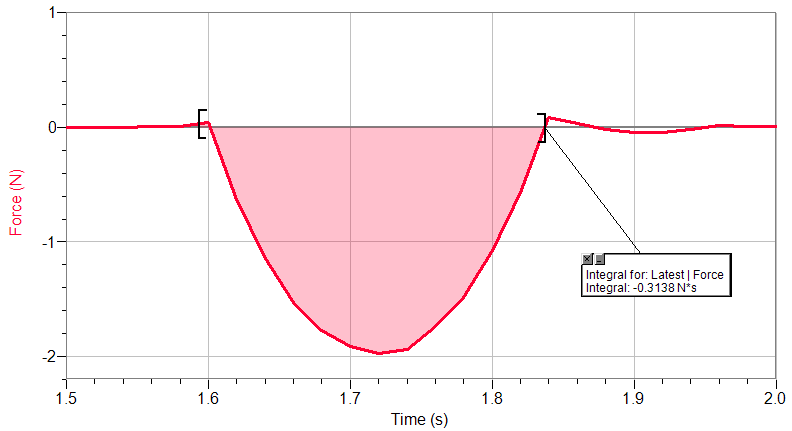
\includegraphics[width=3.2in]{slow_force}
                \caption{Slow force. The impulse measured is \impls{-0.3138}.}
            \end{subfigure}%
            ~
            \begin{subfigure}[t]{0.5\textwidth}
                \centering
                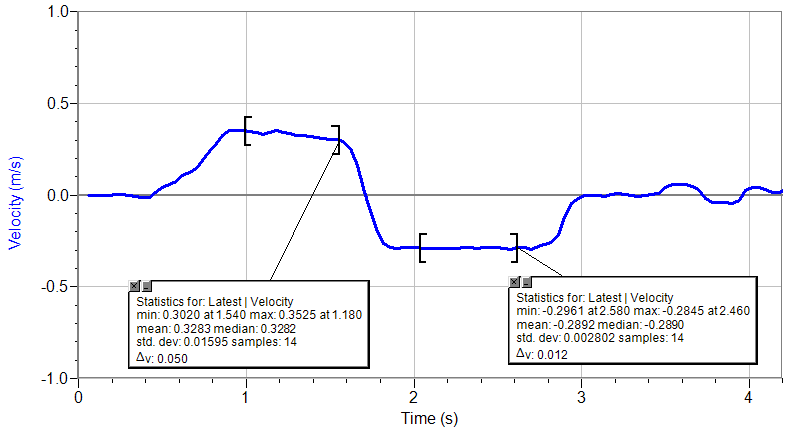
\includegraphics[width=3.2in]{slow_velo}
                \caption{Slow velocity. The initial velocity is \mps{0.3283} with \textsigma\ = \mps{0.0159}, and the final velocity is \mps{-.2890} with \textsigma\ = \mps{0.0028}}
            \end{subfigure}
            \caption{Slow trial measurements.}
        \end{figure}
        %slower
        \begin{figure}[H]
            \begin{subfigure}[t]{0.5\textwidth}
                \centering
                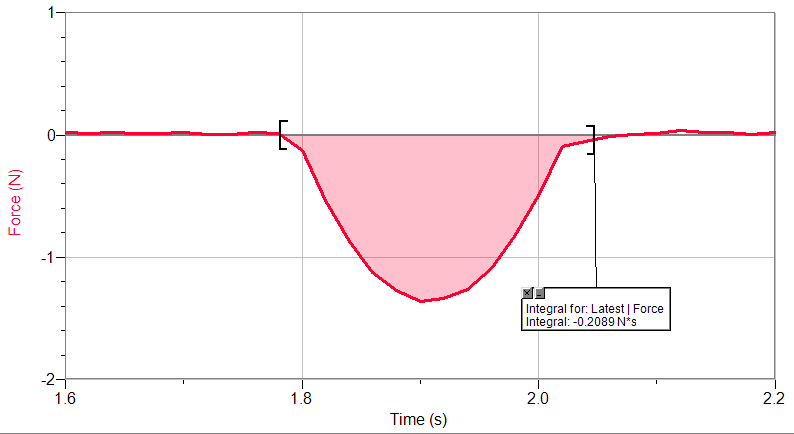
\includegraphics[width=3.2in]{slower_force}
                \caption{Slower force. The impulse measured is \impls{-0.2089}.}
            \end{subfigure}%
            ~
            \begin{subfigure}[t]{0.5\textwidth}
                \centering
                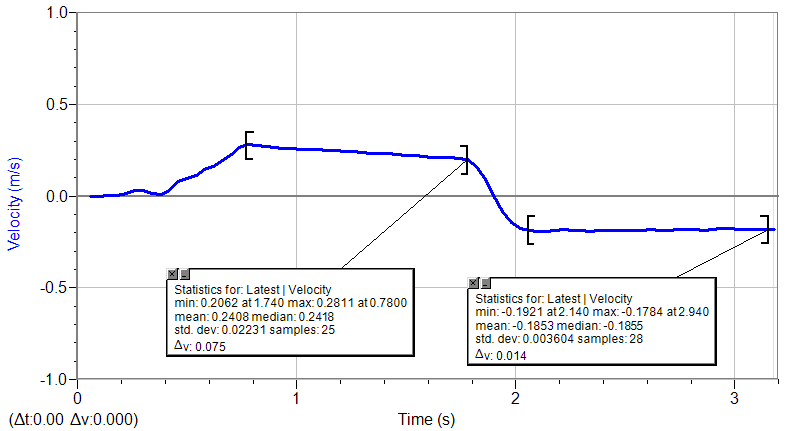
\includegraphics[width=3.2in]{slower_velo}
                \caption{Slower velocity. The initial velocity is \mps{0.2408} with \textsigma\ = \mps{0.0223}, and the final velocity is \mps{-.1853} with \textsigma\ = \mps{0.0004}}
            \end{subfigure}
            \caption{Slower trial measurements.}
        \end{figure}
        %slowest
        \begin{figure}[H]
            \begin{subfigure}[t]{0.5\textwidth}
                \centering
                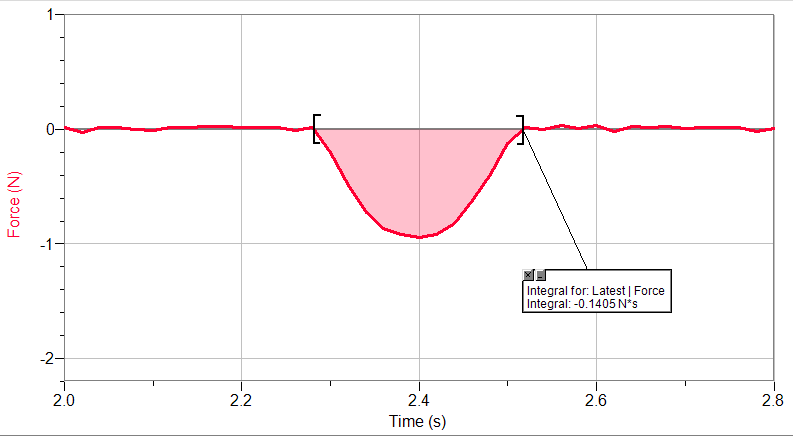
\includegraphics[width=3.2in]{slowest_force}
                \caption{Slowest force. The impulse measured is \impls{-0.1405}.}
            \end{subfigure}%
            ~
            \begin{subfigure}[t]{0.5\textwidth}
                \centering
                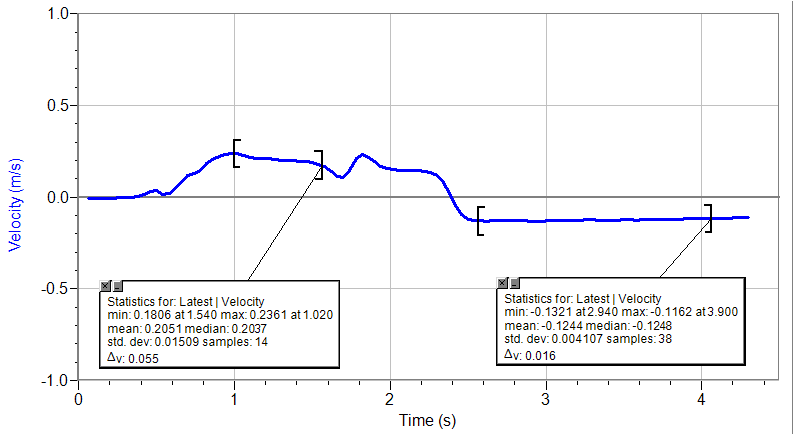
\includegraphics[width=3.2in]{slowest_velo}
                \caption{Slowest velocity. The initial velocity is \mps{0.2051} with \textsigma\ = \mps{0.0151}, and the final velocity is \mps{-.1244} with \textsigma\ = \mps{0.0041}}
            \end{subfigure}
            \caption{Slowest trial measurements.}
        \end{figure}
        ~
        \begin{table}[H]
            \centering
            \caption{Experiment Data}
            \label{tab:1}
            \begin{tabular}{@{} llll @{}}
                \toprule
                Measurement                     &{Slow}             &{Slower}           &{Slowest}\\ \midrule
                Impulse                         &\impls{-0.3138}    &\impls{-0.2089}    &\impls{-0.1405}\\[.4em]
                Initial Velocity                &\mps{0.3283}       &\mps{0.2408}       &\mps{0.2051}\\[.4em]
                Initial Velocity Uncertainty    &\mps{0.0159}       &\mps{0.0223}       &\mps{0.0151}\\[.4em]
                Final Velocity                  &\mps{-0.2890}      &\mps{-0.1853}      &\mps{-0.1244}\\[.4em]
                Final Velocity Uncertainty      &\mps{0.0028}       &\mps{0.0004}       &\mps{.0041}\\[.4em]
                Mass of Cart                    &\kg{0.4975}        &\kg{0.4975}        &\kg{0.4975}\\[.4em]
                Uncertainty of Mass of Cart     &\kg{0.0001}        &\kg{0.0001}        &\kg{0.0001}\\[.4em]
                Change of Momentum              &\mm{-0.3071}       &\mm{-0.2119}       &\kg{-0.1639}\\[.4em]
                Uncertainty on Momentum         &\mm{0.0065}        &\mm{0.0109}        &\mm{0.0054}\\ \bottomrule
            \end{tabular}
        \end{table}
        \item %
            \begin{enumerate}[a)]
                \item For the slow and slower tests, the results matched within the calculated uncertainty.
                The values were \impls{-0.3138} and \mm{-0.3071}, and \impls{-0.2089} and \mm{-0.2119} respectively.
                For the slowest value, the impulse is \impls{-0.1405}, and the change in momentum is \kg{-0.1639} with uncertainty of \mm{0.0054}.
                \item For the most part, the impulse equaled the change in momentum. I believe I should have redone the slowest trial,
                as the graph was inconsistent, and the data collected doesn't match up with what should be happening.
                \item I believe an interesting addition would be to find the spring constant of the force meter.
            \end{enumerate}
    \end{enumerate}
\end{document}